\documentclass[a4paper,12pt]{report}
\usepackage[margin=1in]{geometry} % to change the page dimensions
\usepackage{ctex}
\usepackage{xeCJK}
\usepackage{comment}
\usepackage{amsmath}
\usepackage{amssymb}
\usepackage{amsthm}
%\usepackage{times}
\usepackage{setspace}
% \usepackage{lastpage}
\usepackage{fancyhdr}
\usepackage{graphicx}
%\graphicspath{{fig/}}
\usepackage{wrapfig}
\usepackage{subfigure}
\usepackage{array}  
% \usepackage{fontspec,xunicode,xltxtra}
% \renewcommand{\sfdefault}{cmr}
\usepackage{titlesec}
\usepackage{titletoc}
\usepackage[titletoc]{appendix}
%\usepackage[top=30mm,bottom=30mm,left=20mm,right=20mm]{geometry}
%\usepackage{cite}
\usepackage[backend = biber, style = gb7714-2015, defernumbers=true]{biblatex}
\renewcommand*{\bibfont}{\small}
\addbibresource{reference.bib}
%\usepackage{courier}
\setmonofont{Courier New}
\usepackage{listings}
\lstset{tabsize=4, keepspaces=true,
    xleftmargin=2em,xrightmargin=0em, aboveskip=1em,
    %backgroundcolor=\color{gray!20},  % 定义背景颜色
    frame=none,                       % 表示不要边框
    extendedchars=false,              % 解决代码跨页时,章节标题,页眉等汉字不显示的问题
    numberstyle=\ttfamily,
    basicstyle=\ttfamily,
    keywordstyle=\color{blue}\bfseries,
    breakindent=10pt,
    identifierstyle=,                 % nothing happens
    commentstyle=\color{green}\small,  % 注释的设置
    morecomment=[l][\color{green}]{\#},
    numbers=left,stepnumber=1,numberstyle=\scriptsize,
    showstringspaces=false,
    showspaces=false,
    flexiblecolumns=true,
    breaklines=true, breakautoindent=true,breakindent=4em,
    escapeinside={/*@}{@*/},
}
\usepackage{amsmath}
\usepackage{amsthm}
\newtheorem{theorem}{定理}
\newtheorem{definition}{定义}
\newtheorem{corollary}{推论}
\newtheorem{example}{例}
\usepackage{amsfonts}
%\usepackage{bm}
\usepackage{booktabs} % for much better looking tables
\usepackage{paralist} % very flexible & customisable lists (eg. enumerate/itemize, etc.)
\usepackage{verbatim} % adds environment for commenting out blocks of text & for better verbatim
\usepackage{subfigure} % make it possible to include more than one captioned figure/table in a single float
% These packages are all incorporated in the memoir class to one degree or another...
\usepackage{cases} %equation set
\usepackage{multirow} %use table
\usepackage{algorithm}
\usepackage{algorithmic}
\usepackage{hyperref}
\hypersetup{colorlinks,linkcolor=black,anchorcolor=black,citecolor=black, pdfstartview=FitH,bookmarksnumbered=true,bookmarksopen=true,} % set href in tex & pdf
%\usepackage[framed,numbered,autolinebreaks,useliterate]{mcode} % 插入matlab代码
\XeTeXlinebreaklocale "zh"
\XeTeXlinebreakskip = 0pt plus 1pt minus 0.1pt

\makeatletter
\newenvironment{breakablealgorithm}
  {% \begin{breakablealgorithm}
   \begin{center}
     \refstepcounter{algorithm}% New algorithm
     \hrule height.8pt depth0pt \kern2pt% \@fs@pre for \@fs@ruled
     \renewcommand{\caption}[2][\relax]{% Make a new \caption
       {\raggedright\textbf{\ALG@name~\thealgorithm} ##2\par}%
       \ifx\relax##1\relax % #1 is \relax
         \addcontentsline{loa}{algorithm}{\protect\numberline{\thealgorithm}##2}%
       \else % #1 is not \relax
         \addcontentsline{loa}{algorithm}{\protect\numberline{\thealgorithm}##1}%
       \fi
       \kern2pt\hrule\kern2pt
     }
  }{% \end{breakablealgorithm}
     \kern2pt\hrule\relax% \@fs@post for \@fs@ruled
   \end{center}
  }
\makeatother
%%%%此处break 算法
%---------------------------------------------------------------------
%	页眉页脚设置
%---------------------------------------------------------------------
\fancypagestyle{plain}{
    \pagestyle{fancy}      %改变章节首页页眉
}

\pagestyle{fancy}
\lhead{\kaishu~数据挖掘实验报告~}
%\rhead{\kaishu~xxx}
\cfoot{\thepage}
\titleformat{\chapter}{\centering\zihao{2}\heiti}{第\chinese{chapter}章}{1em}{}
% \titleformat{\chapter*}{\centering\zihao{-1}\heiti}
\begin{comment}
%---------------------------------------------------------------------
%	章节标题设置
%---------------------------------------------------------------------
\titleformat{\chapter}{\centering\zihao{-1}\heiti}{实验\chinese{chapter}}{1em}{}
\titlespacing{\chapter}{0pt}{*0}{*6}
\end{comment}
%---------------------------------------------------------------------
%	摘要标题设置
%---------------------------------------------------------------------
%\renewcommand{\abstractname}{摘要}
\renewcommand{\figurename}{图}
\renewcommand{\tablename}{表}

%---------------------------------------------------------------------
%	参考文献设置
%---------------------------------------------------------------------
%\renewcommand{\bibname}{\zihao{2}{\hspace{\fill}参\hspace{0.5em}考\hspace{0.5em}文\hspace{0.5em}献\hspace{\fill}}}
\renewcommand{\bibname}{参考文献}
\begin{comment}
%---------------------------------------------------------------------
%	引用文献设置为上标
%---------------------------------------------------------------------
\makeatletter
\def\@cite#1#2{\textsuperscript{[{#1\if@tempswa , #2\fi}]}}
\makeatother
\end{comment}
%---------------------------------------------------------------------
%	目录页设置
%---------------------------------------------------------------------
%\renewcommand{\contentsname}{\zihao{-3} 目\quad 录}
\renewcommand{\contentsname}{目录}
\titlecontents{chapter}[0em]{\songti\zihao{-4}}{\thecontentslabel\ }{}
{\hspace{.5em}\titlerule*[4pt]{$\cdot$}\contentspage}
\titlecontents{section}[2em]{\vspace{0.1\baselineskip}\songti\zihao{-4}}{\thecontentslabel\ }{}
{\hspace{.5em}\titlerule*[4pt]{$\cdot$}\contentspage}
\titlecontents{subsection}[4em]{\vspace{0.1\baselineskip}\songti\zihao{-4}}{\thecontentslabel\ }{}
{\hspace{.5em}\titlerule*[4pt]{$\cdot$}\contentspage}

\begin{document}
%---------------------------------------------------------------------
%	封面设置
%---------------------------------------------------------------------
\begin{titlepage}
    \begin{center}
        
    \includegraphics[width=0.60\textwidth]{nk_logo.pdf}\\
    \vspace{10mm}
    \hspace*{\fill} \\
    \textbf{\zihao{1}{数据挖掘实验报告}}\\
    \vspace{\fill}
    
\setlength{\extrarowheight}{3mm}
{\songti\zihao{3}	
\begin{tabular}{rl}
    
    {\makebox[4\ccwd][s]{学\qquad 号:\qquad 2\ 2\ 1\ 3\ 1\ 1\ 7}} & ~\kaishu   \\
    {\makebox[4\ccwd][s]{姓\qquad 名:\qquad 蔡\quad 佳\quad 良}} & ~\kaishu   \\
    {\makebox[4\ccwd][s]{年\qquad 级:\qquad 2\ 0\ 2\ 2\quad 级}} & ~\kaishu   \\
    {\makebox[4\ccwd][s]{学\qquad 院:\qquad 统计与数据科学学院}} & ~\kaishu   \\
    {\makebox[4\ccwd][s]{专\qquad 业:\qquad 统\quad 计\quad 学}} & ~\kaishu   \\
    %{\makebox[4\ccwd][s]{授课教师:}}  & ~\kaishu xxx~教授\\ 
    %{\makebox[4\ccwd][s]{课程助教:}} & ~\kaishu xxx~xxx \\
    {\makebox[4\ccwd][s]{完成日期:}}  & ~\kaishu\quad2\ 0\ 2\ 4年\ 1\ 1月\ 1\ 7日\\ 

\end{tabular}
 }\\[2cm]
%\vspace{\fill}
%\zihao{4}
%使用\LaTeX 撰写于\today
    \end{center}	
\end{titlepage}

%---------------------------------------------------------------------
%  摘要页
%---------------------------------------------------------------------


%---------------------------------------------------------------------
%  目录页
%---------------------------------------------------------------------
\tableofcontents % 生成目录

%---------------------------------------------------------------------
%  绪论
%---------------------------------------------------------------------
\chapter{第一次上机实验(提取图像的纹理特征)}
\section{实验要求}
\begin{itemize}
    \item 给定若干张图像,利用灰度共生矩阵特征或局部二值模式特征对这些图像进行特征提取;
    \item 图象是W * H * 3的矩阵;
    \item 将最终提取到的特征通过plot的形式展示,直观对比不同纹理提取到的特征;
    \item 使用Python编程实现。
\end{itemize}
\section{数据分析与处理}
\par 将图像转化为灰度矩阵。
\section{实验步骤与原理}
\subsection{灰度共生矩阵}
\par 灰度共生矩阵是从$N\times N$的图像$f(x,y)$的灰度为$i$的像素出发,统计与距离为$\delta=(\mathrm{d}x^{2}+\mathrm{d}y^{2})^{1/2}$,灰度为$j$的像素同时出现的概率为,数学表达式为:$$P(i,j,\delta,\theta)=\left\{[(x,y),(x+\mathrm{d}x,y+\mathrm{d}y)]|f(x,y)=i,f(x+\mathrm{d}x,y+\mathrm{d}y)=j\right\},$$
\par 分别考虑$\theta=0^{\circ},45^{\circ},90^{\circ},135^{\circ}$,
\par 当$\theta=0^{\circ}$时,$\mathrm{d}x=1,\mathrm{d}y=0$;
\par 当$\theta=45^{\circ}$时,$\mathrm{d}x=1,\mathrm{d}y=-1$;
\par 当$\theta=90^{\circ}$时,$\mathrm{d}x=0,\mathrm{d}y=-1$;
\par 当$\theta=135^{\circ}$时,$\mathrm{d}x=-1,\mathrm{d}y=-1$。
\subsection{局部二值模式}
\par LBP算子定义为在3*3的窗口内,以窗口中心像素为阈值,将相邻的8个像素的灰度值与其进行比较,若周围像素值大于中心像素值,则该像素点的位置被标记为1,否则为0。这样,3*3邻域内的8个点经比较可产生8位二进制数(通常转换为十进制数即LBP码,共256种),即得到该窗口中心像素点的LBP值,并用这个值来反映该区域的纹理信息(例如亮点和暗点),数学表达式为:
$$LBP=\sum_{p=0}^{P−1} s(g_p−g_c)\cdot 2^p,$$
\par 其中,

\begin{itemize}
    \item $s(x)$是符号函数:
    $$s(x)=\left\{ \begin{array}{rcl}1\quad x\ge 0\\0\quad x<0\end{array}\right.,$$
    \item P 是邻域像素数(通常为 8)。
\end{itemize}
\section{实验结果与分析}
\par 通过两种方法下生成的\href{https://github.com/psa1K/Data_mining_2024/tree/main/datasets/exp1/output}{特征图}可以看出,两类图有明显不同的纹理特征。
\section{实验代码}
\begin{lstlisting}[language=Python]
import os
import numpy as np
import matplotlib.pyplot as plt
import matplotlib as mpl
from PIL import Image, ImageDraw, ImageFont

mpl.rcParams["font.sans-serif"] = ["SimHei"]  # 中文
plt.rcParams["axes.unicode_minus"] = False  # 正负号

# 更改当前工作目录为脚本所在目录
os.chdir(os.path.dirname(os.path.abspath(__file__)))
c_path = "./cloud/"
f_path = "./forest/"

os.makedirs("./output/glcm/", exist_ok=True)  # 创建输出文件夹
os.makedirs("./output/lbp/", exist_ok=True)

c_name = [c_path + i for i in os.listdir(c_path)]
f_name = [f_path + i for i in os.listdir(f_path)]


def show_grey(root=c_name):
    for n, i in enumerate(c_name):
        plt.subplot(2, 5, n + 1)
        img = Image.open(i)
        img = img.convert("L")  # 转为灰度图
        plt.imshow(img, cmap="gray")  # 显示灰度图
        plt.axis("off")  # 不显示坐标轴
    plt.show()


def get_mat(root):
    for n, i in enumerate(root):
        # plt.subplot(2, 5, n + 1)
        img = Image.open(i)
        img = img.convert("L")  # 转为灰度图
        img = np.array(img)  # 转为ndarray
        yield i, img


# 计算灰度共生矩阵(gray-level co-occurrence matrix)
def get_glcm(img, angle=0, distance=1, gray_levels=256):
    # 归一化到0-gray_levels灰度级
    img = (img / (np.max(img) + 1e-5) * (gray_levels - 1)).astype(int)
    h, w = img.shape  # 获取图像的尺寸
    glcm = np.zeros((gray_levels, gray_levels), dtype=np.int64)

    for i in range(h):
        for j in range(w):
            match angle:
                case 0:
                    if j + distance < w:
                        glcm[img[i, j], img[i, j + distance]] += 1
                case 90:
                    if i + distance < h:
                        glcm[img[i, j], img[i + distance, j]] += 1
                case 45:
                    if i + distance < h and j + distance < w:
                        glcm[img[i, j], img[i + distance, j + distance]] += 1
                case 135:
                    if i + distance < h and j - distance >= 0:
                        glcm[img[i, j], img[i + distance, j - distance]] += 1

    glcm = glcm / np.sum(glcm)  # 归一化
    return glcm


# 绘制灰度共生矩阵
def get_glcm_fig(root, angles=[0, 45, 90, 135]):
    for i, img in get_mat(root):
        glcms = []  # 存储各角度的 GLCM 图像
        for angle in angles:
            glcm = get_glcm(img, angle=angle)
            glcm = (glcm / glcm.max() * 255).astype(np.uint8)
            glcms.append((Image.fromarray(glcm), f"Angle: {angle}°"))  # 保存图像和标题

        # 计算单张 GLCM 图像的大小
        width, height = glcms[0][0].size
        title_height = 20  # 为标题预留的高度

        # 2x2 布局,标题增加额外空间
        canvas = Image.new("L", (2 * width, 2 * (height + title_height)), "white")

        draw = ImageDraw.Draw(canvas)
        font = ImageFont.load_default()

        for idx, (glcm, title) in enumerate(glcms):
            x_offset = (idx % 2) * width
            y_offset = (idx // 2) * (height + title_height)

            text_bbox = draw.textbbox((0, 0), title, font=font)
            text_width = text_bbox[2] - text_bbox[0]
            text_x = x_offset + (width - text_width) // 2
            draw.text((text_x, y_offset), title, fill="black", font=font)

            canvas.paste(glcm, (x_offset, y_offset + title_height))

        canvas.save(f"./output/glcm/{i}")


# 计算局部二值模式(local binary pattern)
def get_lbp(img):
    h, w = img.shape  # 获取图像的尺寸
    lbp = np.zeros((h - 2, w - 2), dtype=np.int64)  # 忽略边缘像素
    for i in range(1, h - 1):
        for j in range(1, w - 1):
            center = img[i, j]
            neighbors = [
                img[i, j - 1],
                img[i + 1, j - 1],
                img[i + 1, j],
                img[i + 1, j + 1],
                img[i, j + 1],
                img[i - 1, j + 1],
                img[i - 1, j],
                img[i - 1, j - 1],
            ]
            code = 0
            for idx, neighbor in enumerate(neighbors):
                if neighbor > center:
                    code += 2**idx
            lbp[i - 1, j - 1] = code
    return lbp


# 绘制局部二值模式
def get_lbp_fig(root):
    for i, img in get_mat(root):
        lbp = get_lbp(img)
        Image.fromarray(lbp.astype(np.uint8)).save(f"./output/lbp/{i}")


def main():
    roots = [c_name, f_name]
    for root in roots:
        get_glcm_fig(root)
        get_lbp_fig(root)


if __name__ == "__main__":
    main()

\end{lstlisting}
\clearpage
\chapter{第二次上机实验(垂直平分分类器)}
\section{实验要求}
\begin{itemize}
    \item 由\href{https://github.com/mercier111/Data_mining_2021/blob/main/data/2021_0325/data/train.txt}{训练数据},训练一个垂直平分分类器;
    \item 对\href{https://github.com/mercier111/Data_mining_2021/blob/main/data/2021_0325/data/test.txt}{测试数据}进行分类;
    \item 使用Python编程实现。
\end{itemize}
\section{数据分析与处理}
\par 测试集与训练集均为已分类的二维数据。
\section{实验步骤与原理}
训练集中两类数据的均值分别为记为$m_{1}$和$m_{2}$,
则垂直平分形式的线性分类器为
$$g(\boldsymbol{x})=(m_{1})^{\prime}(\boldsymbol{x}-(m_{1}-m_{2})/2),$$
决策面方程为$$g(\boldsymbol{x})=0,$$
其中$\boldsymbol{x}$为向量。
\par 当$g(\boldsymbol{x})>0$时,决策为“1”类,否则为“2”类。
\section{实验结论与分析}
\par 图~\ref{2.1} 展示了训练集与决策面的可视化图,图~\ref{2.2} 展示了测试集与决策面可视化图。进而可以计算出模型的准确率(accuracy),精确率(precision),召回率(recall)和 F1得分的值分别为99.25\%,99.00\%,99.50\%,99.25\%(保留两位小数)。说明模型的预测性能表现优异。
\begin{figure}[htbp]
    \centering
    \begin{minipage}{0.42\textwidth}
        \centering
        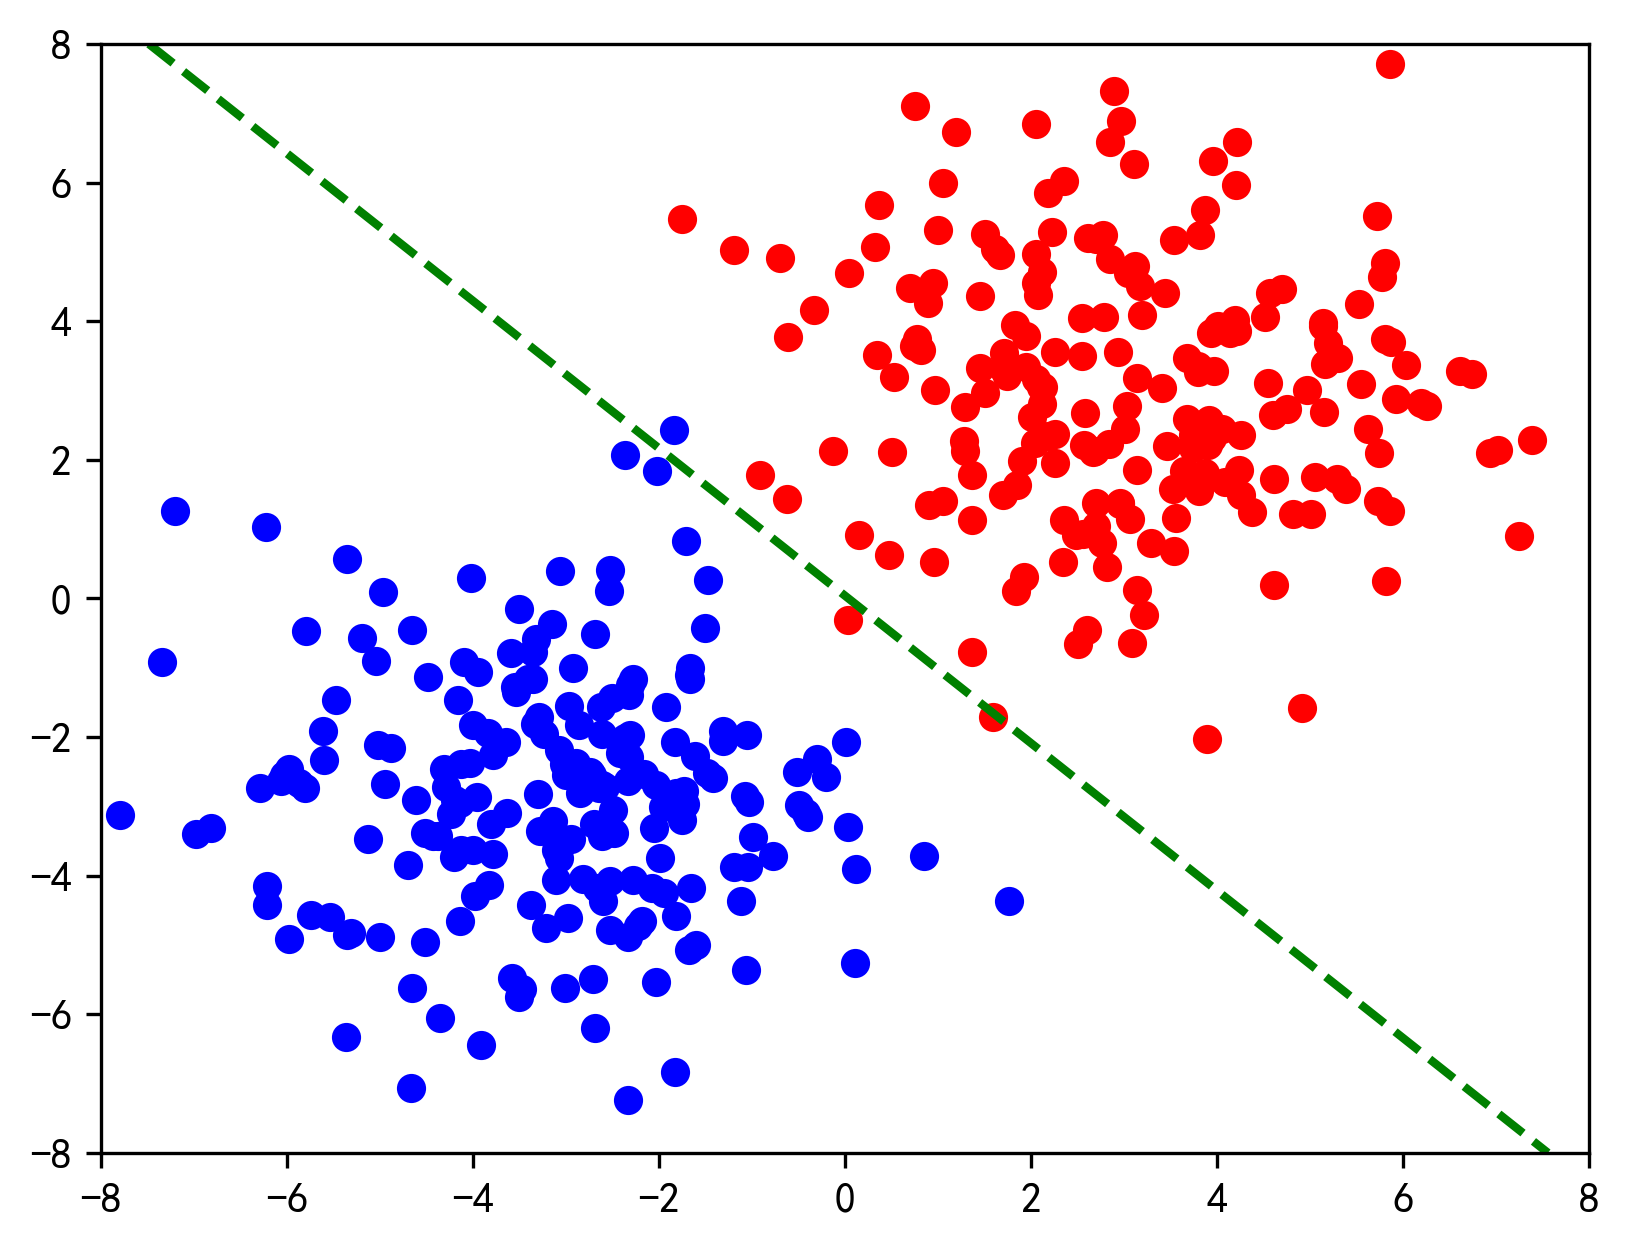
\includegraphics[width=\textwidth]{../datasets/exp2/output/train.png}
        \caption{训练集与决策面}
        \label{2.1}
    \end{minipage}
    \hfill
    \begin{minipage}{0.42\textwidth}
        \centering
        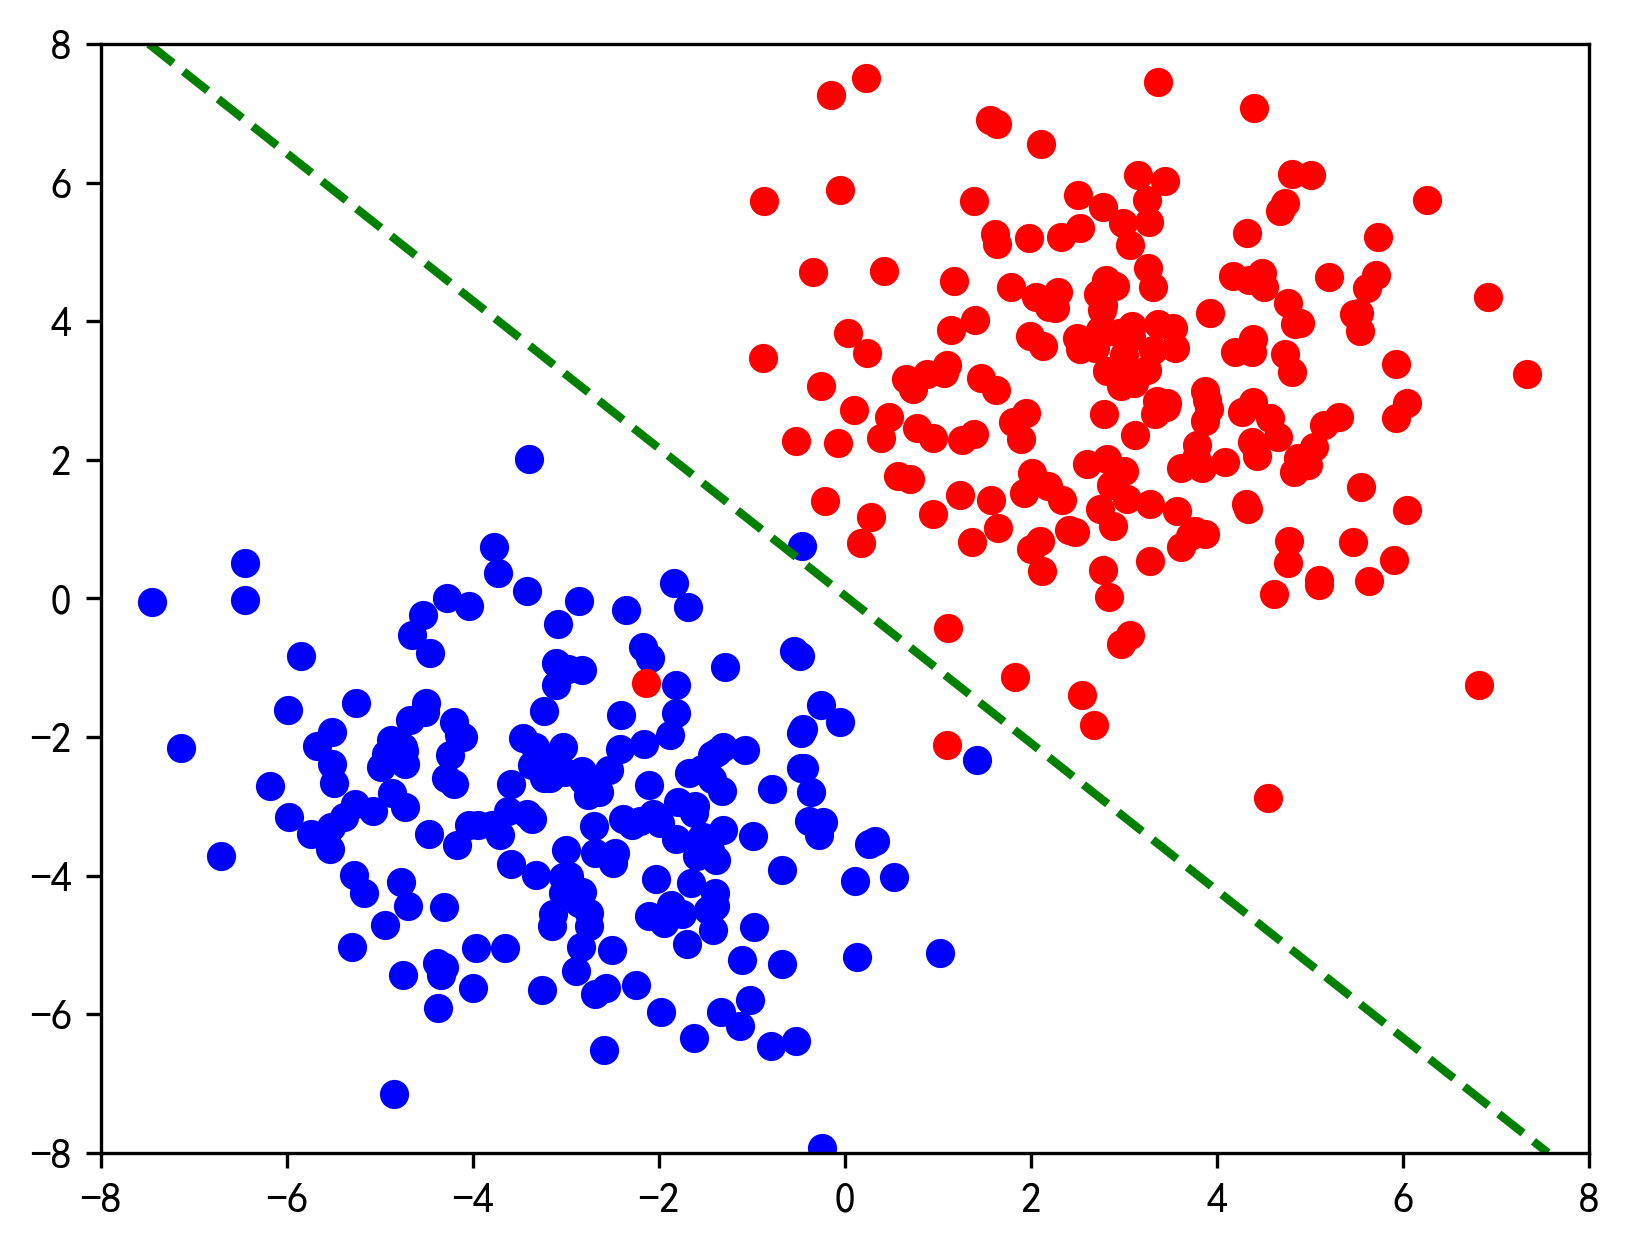
\includegraphics[width=\textwidth]{../datasets/exp2/output/test.png}
        \caption{测试集与决策面}
        \label{2.2}
    \end{minipage}
    \label{fig:train_test_comparison}
\end{figure}
\section{实验代码}
\begin{lstlisting}[language=Python]
import numpy as np
import pandas as pd
import matplotlib.pyplot as plt
import matplotlib as mpl
import os

mpl.rcParams["font.sans-serif"] = ["SimHei"]  # 中文
plt.rcParams["axes.unicode_minus"] = False  # 负号
os.chdir(os.path.dirname(os.path.abspath(__file__)))  # 更改当前工作目录为脚本所在目录

train_path = "data/train.txt"
test_path = "data/test.txt"


def train(data):
    mean = data.groupby("Label").mean()
    m_1 = mean.loc[1]
    m_2 = mean.loc[2]
    point = (m_1 + m_2) / 2
    slope = m_1 - m_2
    return point, slope


def test(data, point, slope):
    data["Predict"] = np.where(
        (data.X - point.X) * slope.X + (data.Y - point.Y) * slope.Y > 0, 1, 2
    )
    data.to_csv("output/test_predict.csv")
    return data


def plot(data, point, slope, filename):
    plt.axline(
        point,
        slope=-slope.X / slope.Y,
        color="green",
        linewidth=2,
        linestyle="--",
        label="Perpendicular Bisector Classifier",
    )
    color = ["r", "b"]
    for _, i in data.iterrows():
        x, y, c = i.iloc[0], i.iloc[1], color[int(i.iloc[2]) - 1]
        plt.scatter(x, y, color=c)
    plt.xlim(-8, 8)
    plt.ylim(-8, 8)
    plt.axis("off")
    plt.savefig(filename, dpi=300, bbox_inches="tight")
    # plt.show()
    plt.close()


def evaluate(data):
    TP = 0
    TN = 0
    FP = 0
    FN = 0
    for _, i in data.iterrows():
        if i.iloc[2] == i.iloc[3]:
            if i.iloc[2] == 1:
                TP += 1
            else:
                TN += 1
        else:
            if i.iloc[2] == 1:
                FP += 1
            else:
                FN += 1
    accuracy = (TP + TN) / (TP + TN + FP + FN)
    precision = TP / (TP + FP)
    recall = TP / (TP + FN)
    F1 = 2 * precision * recall / (precision + recall)
    print("accuracy:", accuracy)
    print("precision:", precision)
    print("recall:", recall)
    print("F1 score:", F1)


def main():
    train_data = pd.read_csv(train_path, index_col=0)
    test_data = pd.read_csv(test_path, index_col=0)
    point, slope = train(train_data)
    # 绘制测试集与决策界
    plot(train_data, point, slope, "./output/train.png")
    # 绘制训练集与决策界
    plot(test_data, point, slope, "./output/test.png")
    test_data = test(test_data, point, slope)
    # 评估测试结果
    evaluate(test_data)


if __name__ == "__main__":
    main()

\end{lstlisting}
\clearpage
\chapter{第三次上机实验(使用朴素贝叶斯方法进行预测)}
\section{实验要求}
\begin{itemize}
    \item 给定一定时间内的犯罪数据集,使用朴素贝叶斯方法进行犯罪类型预测;
    \item 使用Python编程实现。
\end{itemize}
\section{数据分析与处理}
\label{3.2}
\par 原始数据包括Dates, Category, Descript, DayOfWeek, PdDistrict。其中Category是我们要尽心预测的对象,我们对其进行编码,然后我们对Dates, DayOfWeek, PdDistrict进行one-hot编码,利用TD-IDF特征从Descript中提取关键词并进行编码。
\section{实验步骤与原理}
\par 给定特征 $\boldsymbol{x}=(x_{1},x_{2},\cdots,x_{n})$和类别$\boldsymbol{v}=(v_{1},v_{2},\cdots,v_{m})$。在分类任务中,我们想要找到使得$P(v|\boldsymbol{x})$最大的$v$。利用贝叶斯公式
$$P(v|\boldsymbol{x})=\frac{P(\boldsymbol{x}|v)P(v)}{P(\boldsymbol{x})},$$
又$P(x)$为定值,则我们比较$P(\boldsymbol{x}|v)P(v)$即可。
\par 在朴素贝叶斯中,我们假设特征$x_{1},x_{2},\cdots,x_{n}$之间是相互独立的,即
$$
P(\boldsymbol{x}|v)=\prod_{i=1}^{n}P(x_{i}|v).
$$
\par 则使得$P(v|\boldsymbol{x})$最大的
$$
v=\mathop{\arg\max}\limits_{v_{j}}P(v_{j})\prod_{i=1}^{n}P(x_{i}|v_{j})
$$
\begin{figure}[htbp]
    \centering
    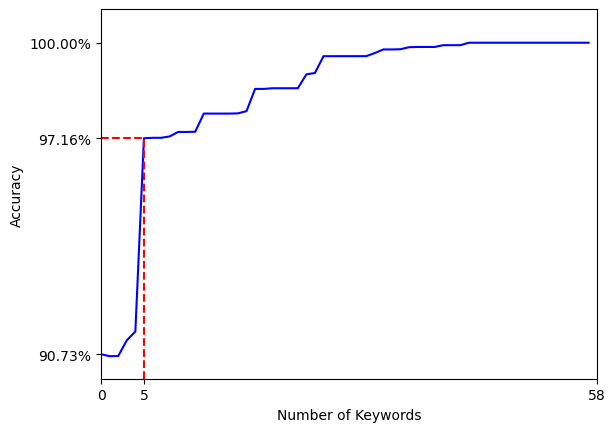
\includegraphics[width=\textwidth]{../datasets/exp3/accuracy.png}
    \caption{测试集上的准确率与关键词个数关系图}
    \label{3.1}
    \hfill
\end{figure}
\section{实验结论与分析}
\par 根据TF-IDF值对每一个Descript选取一个关键词,选取出现频率最高的k个关键词进行模型拟合,在测试集上的准确率如图~\ref{3.1} 所示。为了防止模型过拟合并保证其泛化能力,选取频率最高的前5个关键词。
\par 考虑测试集和训练集Category中DRUG/NARCOTIC类数据分别占据90.79\%和89.81\%,为不均衡数据,本实验模型的分类正确率达到了97.16\%,效果较好。
\section{实验代码}
\begin{lstlisting}[language=Python]
import os
import pandas as pd
from sklearn import preprocessing
from sklearn.naive_bayes import BernoulliNB
from sklearn.metrics import accuracy_score
from sklearn.feature_extraction.text import TfidfVectorizer
import matplotlib.pyplot as plt

os.chdir(os.path.dirname(os.path.abspath(__file__)))  # 更改当前工作目录为脚本所在目录

train_path = "train.csv"
test_path = "test.csv"


def keyword_extract(path="train.csv"):
    df = pd.read_csv(path)
    vectorizer = TfidfVectorizer(stop_words="english", token_pattern=r"(?u)\b\w+\b")
    tfidf = pd.DataFrame(
        vectorizer.fit_transform(df["Descript"]).toarray(),
        columns=vectorizer.get_feature_names_out(),
    )
    keywords = tfidf.idxmax(axis=1)
    keywords = keywords.value_counts(normalize=True).index.str.upper().tolist()
    return keywords


def Pre_Process(path, keywords):
    df = pd.read_csv(path)

    # 将Category进行整数编码
    encoder = preprocessing.LabelEncoder()
    crime_type_encode = encoder.fit_transform(df["Category"])

    # 将时间进行one-hot编码
    hour = pd.to_datetime(df["Dates"]).dt.hour
    hour = pd.get_dummies(hour)
    day = pd.get_dummies(df["DayOfWeek"])

    # 将所属警区进行one-hot编码
    police_district = pd.get_dummies(df["PdDistrict"])

    # 利用 TF-IDF 特征进行编码
    matrix = pd.DataFrame(0, index=df.index, columns=keywords)
    for keyword in keywords:
        matrix[keyword] = df["Descript"].apply(
            lambda x: True if keyword in x else False
        )

    # 将特征合并
    data = pd.concat([hour, day, police_district, matrix], axis=1)
    data["Crime type"] = crime_type_encode

    # Feature names are only supported if all input features have string names
    data.columns = data.columns.astype(str)
    return data


keywords = keyword_extract()
acc = []
for k in range(0, len(keywords) + 1):
    train = Pre_Process(train_path, keywords[:k])
    test = Pre_Process(test_path, keywords[:k])
    # 训练模型
    model = BernoulliNB()
    model.fit(train.drop("Crime type", axis=1), train["Crime type"])

    # 预测结果
    pred = model.predict(test.drop("Crime type", axis=1))
    acc.append(
        accuracy_score(test["Crime type"], pred),
    )

# plot
plt.plot(range(0, len(keywords) + 1), acc, color="b")
plt.xlabel("Number of Keywords")
plt.ylabel("Accuracy")
points = [(0, acc[0]), (5, acc[5]), (len(acc), acc[len(acc) - 1])]
xticks = [x for x, _ in points]
yticks = [y for _, y in points]
plt.xticks(xticks, [f"{x}" for x in xticks])
plt.yticks(yticks, [f"{y * 100:.2f}%" for y in yticks])
plt.plot([points[1][0], points[1][0]], [0.90, points[1][1]], color="r", linestyle="--")
plt.plot([0.00, points[1][0]], [points[1][1], points[1][1]], color="r", linestyle="--")
plt.xlim(0, len(keywords) + 1)
plt.ylim(0.90, 1.01)
# plt.show()
plt.savefig("accuracy.png", bbox_inches="tight")
\end{lstlisting}
\clearpage
\chapter{第四次上机实验(使用决策树进行预测)}
\section{实验要求}
\begin{itemize}
    \item 给定一定时间内的犯罪数据集,使用决策树方法进行犯罪类型预测;
    \item 使用Python编程实现。
\end{itemize}
\section{数据分析与处理}
\par 同~\ref{3.2}\ 节。
\section{实验步骤与原理}
\par 本试验采用CART算法,其不纯度(Gini系数)定义如下:
$$
\mathrm{Gini}=1-\sum_{i=1}^{N}p_{i}^{2},
$$
其中$p_{i}$是每个类$i$的概率,$N$是类别总数。信息增益定义为依某个特征进行分类前后的不纯度之差,选择使得信息增益最高的特征。
\section{实验结论与分析}
\par 根据TF-IDF值对每一个Descript选取一个关键词,选取出现频率最高的k个关键词进行模型拟合,在测试集上的准确率如图~\ref{4.1} 所示。可以看出决策树的训练与大部分频率较高的关键词并无较大帮助,部分频率较低的关键词反而可以很好地减少决策树的深度。我们选取所有关键词进行模型训练,最终决策树如图~\ref{4.2},训练集上的准确率达到了100\%。
\begin{figure}[htbp]
    \centering
    \begin{minipage}{0.42\textwidth}
        \centering
        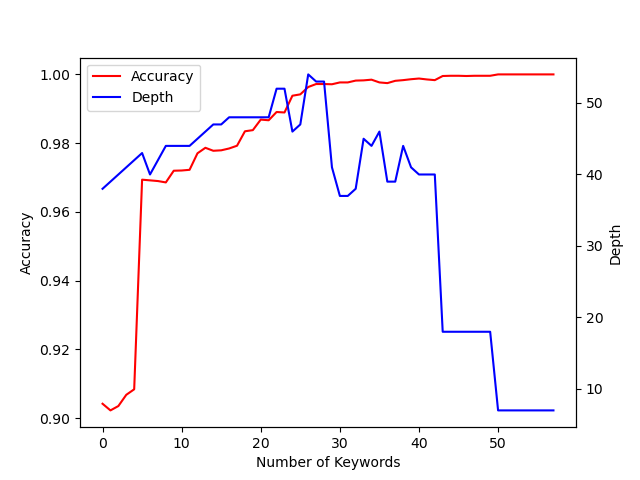
\includegraphics[width=\textwidth]{../datasets/exp4/accuracy+depth.png}
        \caption{决策树深度和测试集上的准确率和与关键词个数关系图}
        \label{4.1}
    \end{minipage}
    \hfill
    \begin{minipage}{0.42\textwidth}
        \centering
        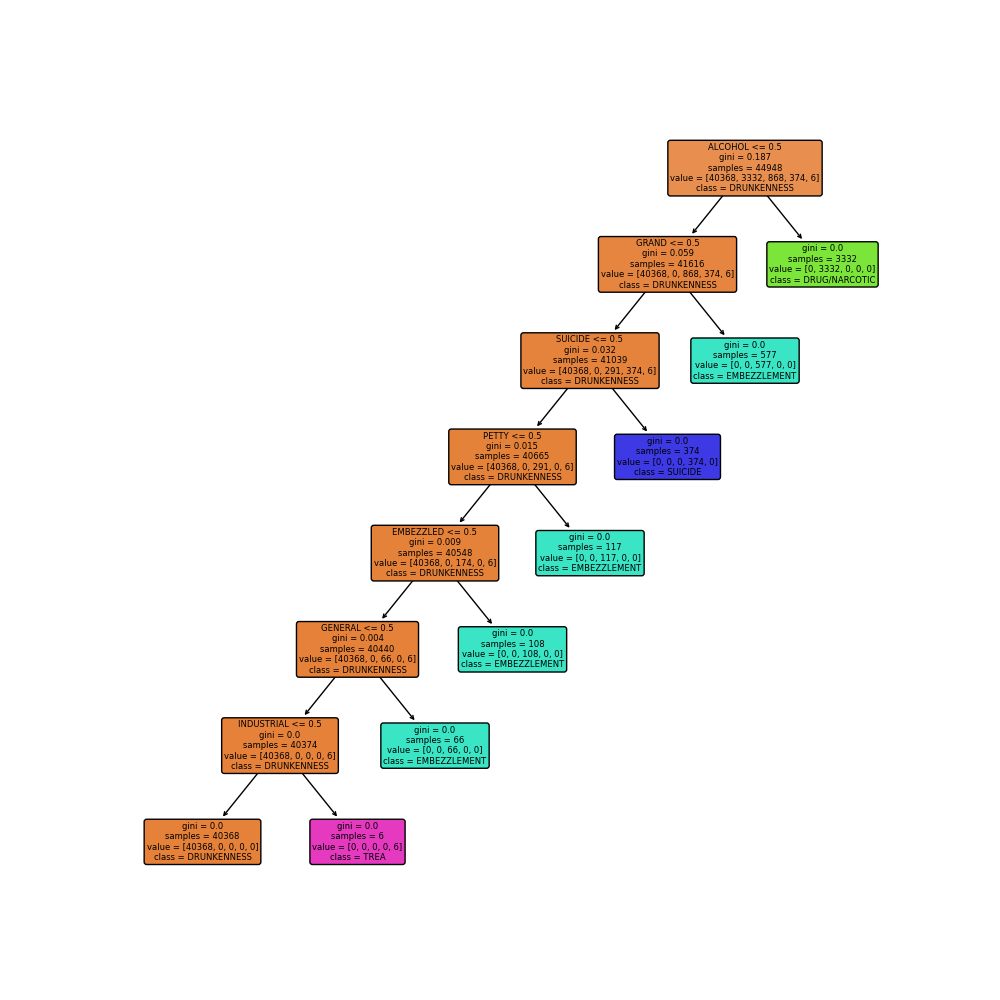
\includegraphics[width=\textwidth]{../datasets/exp4/decision_tree.png}
        \caption{决策树可视化图(Depth=7)}
        \label{4.2}
    \end{minipage}
    \label{fig:train_test_comparison}
\end{figure}
\section{实验代码}
\begin{lstlisting}[language=Python]
import os
import pandas as pd
import matplotlib.pyplot as plt
from sklearn import preprocessing
from sklearn.metrics import accuracy_score
from sklearn.feature_extraction.text import TfidfVectorizer
from sklearn.tree import DecisionTreeClassifier, plot_tree


os.chdir(os.path.dirname(os.path.abspath(__file__)))  # 更改当前工作目录为脚本所在目录

train_path = "train.csv"
test_path = "test.csv"


def keyword_extract(path="train.csv"):
    df = pd.read_csv(path)
    vectorizer = TfidfVectorizer(stop_words="english", token_pattern=r"(?u)\b\w+\b")
    tfidf = pd.DataFrame(
        vectorizer.fit_transform(df["Descript"]).toarray(),
        columns=vectorizer.get_feature_names_out(),
    )
    keywords = tfidf.idxmax(axis=1)
    keywords = keywords.value_counts(normalize=True).index.str.upper().tolist()
    return keywords


def Pre_Process(path, keywords):
    df = pd.read_csv(path)

    # 将Category进行整数编码
    encoder = preprocessing.LabelEncoder()
    crime_type_encode = encoder.fit_transform(df["Category"])

    # 将时间进行one-hot编码
    hour = pd.to_datetime(df["Dates"]).dt.hour
    hour = pd.get_dummies(hour)
    day = pd.get_dummies(df["DayOfWeek"])

    # 将所属警区进行one-hot编码
    police_district = pd.get_dummies(df["PdDistrict"])

    # 利用 TF-IDF 特征进行编码
    matrix = pd.DataFrame(0, index=df.index, columns=keywords)
    for keyword in keywords:
        matrix[keyword] = df["Descript"].apply(
            lambda x: True if keyword in x else False
        )

    # 将特征合并
    data = pd.concat([hour, day, police_district, matrix], axis=1)
    data["Crime type"] = crime_type_encode

    # Feature names are only supported if all input features have string names
    data.columns = data.columns.astype(str)
    return data


keywords = keyword_extract()
acc = []
depth = []
for k in range(0, len(keywords) + 1):
    train = Pre_Process(train_path, keywords[:k])
    test = Pre_Process(test_path, keywords[:k])
    # 训练模型
    model = DecisionTreeClassifier()
    model.fit(train.drop("Crime type", axis=1), train["Crime type"])
    # 预测结果
    y_pred = model.predict(test.drop("Crime type", axis=1))
    acc.append(accuracy_score(test["Crime type"], y_pred))
    depth.append(model.get_depth())

# plot
fig, ax1 = plt.subplots()
ax1.set_xlabel("Number of Keywords")
ax1.set_ylabel("Accuracy")
ax1.plot(range(0, len(keywords) + 1), acc, color="r", label="Accuracy")
ax1.tick_params(axis="y")
# 创建第二个坐标轴共享x轴
ax2 = ax1.twinx()
ax2.set_ylabel("Depth")
ax2.plot(range(0, len(keywords) + 1), depth, color="b", label="Depth")
ax2.tick_params(axis="y")
# 显示图例
lines, labels = ax1.get_legend_handles_labels()
lines2, labels2 = ax2.get_legend_handles_labels()
ax1.legend(lines + lines2, labels + labels2, loc="upper left")
# plt.show()
plt.savefig("accuracy+depth.png")
# 绘制决策树

plt.figure(figsize=(10, 10))
plot_tree(
    model,
    filled=True,
    rounded=True,
    class_names=list(pd.read_csv(train_path)["Category"].unique()),
    feature_names=list(train.drop("Crime type", axis=1).columns),
)
plt.savefig("decision_tree.png")

\end{lstlisting}
\clearpage
\chapter{第五次上机实验}
\section{实验要求}
\section{数据分析与处理}
\section{实验步骤与原理}
\section{实验结论与分析}
\section{实验代码}
\printbibliography

\end{document}